\documentclass[11pt, oneside]{article}   	% use "amsart" instead of "article" for AMSLaTeX format
\usepackage{geometry}                		% See geometry.pdf to learn the layout options. There are lots.
\geometry{letterpaper}                   		% ... or a4paper or a5paper or ... 
%\geometry{landscape}                		% Activate for for rotated page geometry
%\usepackage[parfill]{parskip}    		% Activate to begin paragraphs with an empty line rather than an indent
\usepackage{graphicx}				% Use pdf, png, jpg, or eps§ with pdflatex; use eps in DVI mode
							% TeX will automatically convert eps --> pdf in pdflatex		
\usepackage{amssymb}
\usepackage{hyperref}
\usepackage{listings}

\newcommand{\UB}{USiBeacon} %Use "\UB\" to insert USiBeacon.

\title{USiBeacon}
\author{Ciani Andrea, D'Avico Simone, Gili Daniele}
%\date{}							% Activate to display a given date or no date

\begin{document}
\maketitle
\begin{figure}[htbp]
\begin{center}

\includegraphics[scale=0.5]{img/logo.png}
\end{center}
\end{figure}

\pagebreak
\tableofcontents

% 1. Introduction/ Motivation Scenario

% 2. Prototype Description

% 3. Detailed Hardware & Software Description
\section{Apple iBeacon Technology}

% Spiegare cos'� e come funziona a grandi linee con bt 4.0

\subsection{Reading the iBeacon signal}

% major, minor etc... e come abbiamo fatto
\pagebreak

\section{Indoor Localisation}\label{IndoorLocalisation}\label{indoorlocalisation}
Wikipedia provides a very good introduction about what the Indoor Localisation is and related problem:\\

\emph{``An indoor positioning system (IPS) is a solution to locate objects or people inside a building using radio waves, magnetic fields, acoustic signals, or other sensory information collected by mobile devices.There is currently no de facto standard for an IPS systems design. Nevertheless, there are several commercial systems on the market.}\\

\emph{Instead of using satellites, IPS solutions rely on different technologies, including distance measurement to nearby anchor nodes (nodes with known positions, e.g., WiFi access points), magnetic positioning, dead reckoning. They either actively locate mobile devices and tags or provide ambient location or environmental context for devices to get sensed. The localized nature of an IPS has resulted in design fragmentation, with systems making use of various optical,radio, or even acoustic technologies.}\\

\emph{System designs must take into account that at least three independent measurements are needed to unambiguously find a location (see trilateration). For smoothing to compensate for stochastic (unpredictable) errors there must be a sound method for reducing the error budget significantly. The system might include information from other systems to cope for physical ambiguity and to enable error compensation."}\\

Developing the indoor localisation for our system we faced exactly the problems described in Wikipedia.\\

\subsection{Our first implementation}

We started developing our personal solution using only one beacon, positioned in the center of the room. Then we measured the power loss depending to the distance to the beacon (in terms of db, decibels). When we found the average signal quality a device has inside and outside a specific room we could ``guess" where it was. If, for instance, a dice has a signal strength between 5 and 15 db when it is inside the room, then if the signals is less the 5 the device \emph{should} be outside.\\

The problem about this first implementation was the hight imprecision on the edge of the room. It was quite impossible to distinguish about a device that is close to the door with lots if people inside the room, respect to one that is outside the room but with an empty lecture room.\\

\subsection{Our second implementation}

The second implementation we tried was using multiple beacons. In that case we had more information about the position and we could better guess about the position of the student respect to the lecture room.\\

In this implementation we tried to use less beacon possible for a triangulation, that means: three. The idea behind this solution is quite simple and intuitive. We position three beacons inside the room and by calculating the distance the device has respect to each of them we can try to figure out where it is inside the room.\\

\begin{figure}[htbp]
\begin{center}
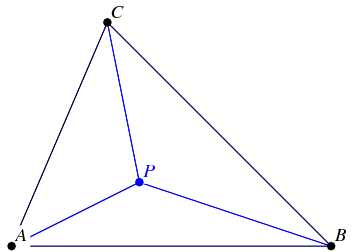
\includegraphics[scale=0.5]{img/triangulation.png}
\caption{The triangulation idea.}
\label{triangulation}
\end{center}
\end{figure}

Even with this solution we had lots of troubles about the precision of the localisation. It wasn't easy to determine with enough precision the position of a device close to the entering/exit doors and how much a user is close to each wall (maybe someone is trying to ``cheat" sticking the device close to a wall).
From this idea we thought that, since every room has four walls, the best idea was to triangulate the position using not three beacons but four of them.\\

\subsection{Our third implementation}
In this implementation we move closer to the implementation adopted by the Estimote's engineers: using four beacons, one for each wall of the room.\\

In fact we figured out that the increased a lot the localisation precision with this last implementation. By positioning a beacon in the center of each wall we could triangulate better the final position.\\

Even if we improved a lot the quality of the tracking there still were mainly two issues:
\begin{itemize}
\item In non-controlled environments, where you can find metals, and other objects that affect the signal, the received signal strength of the beacons changes so often that it seems impossible to get error range below 5 meters.
\item Depending on the way that the user is handling the receiver device, the readings can change a lot as well. If the user puts his/her hand over the bluetooth antenna, then the algorithm will have low signals as input, and thus the beacons will supposed to be very far from the device. See this image to see the precise location of the Bluetooth antenna.
\end{itemize}

\begin{figure}[htbp]
\begin{center}
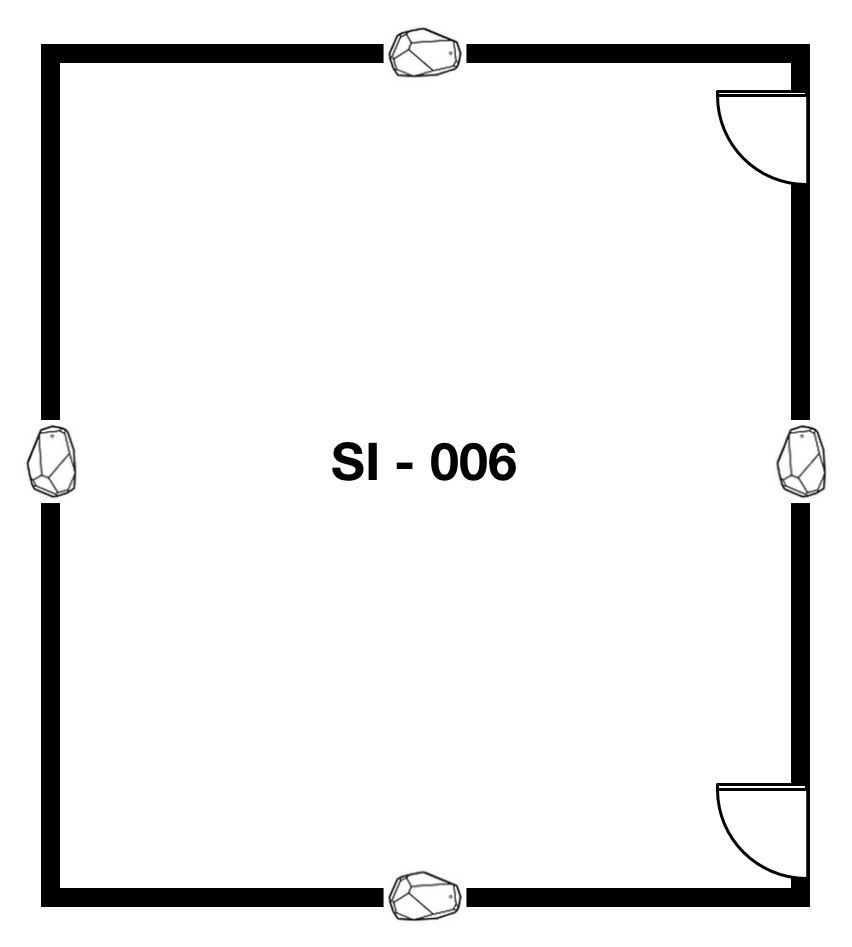
\includegraphics[scale=0.5]{img/room_beacon.png}
\caption{The final result with a triangulation done using three beacons.}
\label{room_beacon}
\end{center}
\end{figure}

\subsection{Our final implementation}
Since we moved closer and closer to the implementation adopted by Estimote we concluded that the best solution was to move to that implementation using the Estimote Frameworks (see \ref{estimoteframework}), available for free in the Estimote website. It uses the same idea we had in the third implementation but adds more then a year of refinement about error correction, wireless noise detection and reduction, as well as the possibility to map the position of each beacon respect to the others by counting the distance between them using an ad-hoc app developed by the Estimote.
\pagebreak

\section{Estimote Framework and Hardware}
% TODO: INSERT REFERENCE TO IBEACON TECHNOLOGY
Estimote is a polish company that develops small wireless sensor implementing the iBeacon \ref{iBeacon} technology providing along the sensors an effective and reliable framework for mobile devices like iOS and Android\footnote{At this time the Android framework is not been released yet}.\\

Estimote Beacons are so small and lightweight that you can attach them to any location or object. They broadcast tiny radio signals which your smartphone can receive and interpret, unlocking micro-location and contextual awareness.\\

\begin{figure}[htbp]
\begin{center}
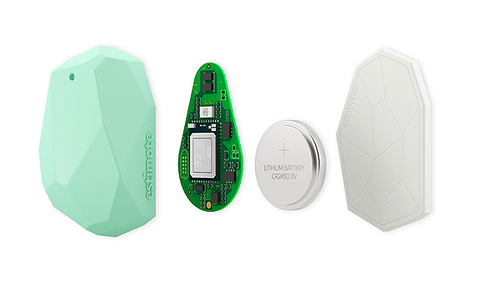
\includegraphics[width=\textwidth]{img/estimotebeacon.png}
\caption{An Estimote sticker cutaway}
\label{estimotesticker}
\end{center}
\end{figure}

With the Estimote SDK, apps on the smartphone are able to understand their proximity to nearby locations and objects, recognising their type, ownership, approximate location, temperature and motion.\\

We used these capabilities in \UB\ to develop a solution that localise a user in an indoor environment and recognise when he/she is inside or outside a specific region (the lecture's room).

\subsection{The framework}\label{estimoteframework}
The Estimote framework is build on the Core Location framework made by Apple and updated on 2014 to support the iBeacon \ref{iBeacon} technology.\\

Estimote develop this framework to wrap the Apple standard indoor functionality and extend the power of localisation by adding the support to the Estimote stickers and their functionality (such as the temperature, the signal power, the identifiers and the connection to the Estimote Cloud).\\

One of the main feature the Estimote engineers focused on is the accuracy of the indoor localisation. The frameworks provides additional support for developers that want to implement their custom localisation in the software, helping to avoid the problems that come from signals noise, peoples in the room, nearby wireless waves etc... (see \ref{indoorlocalisation}). Even if there aren't much information about \emph{how} Estimote is able to improve the quality of the localisation, it seems that they choose an higher frequency for the signal broadcast (from 1Hz specified by Apple in the iBeacon protocol to 5Hz) and a different refresh rate for their devices (less that 1s, maximum limit imposed by the iBeacon). For these reason a proprietary framework between the application and the Estimote devices is quite mandatory.

%TODO: INSERT REFERENCE HERE TO THE CHAPTER ABOUT THE TRIANGULATION PROBLEM.
\pagebreak
% 4. Measurements & Results

\section{The iPhone Application}
The two main important aspect about our project was \textbf{how well the system works} and \textbf{how much easy it is to use}. For this second reason we chose to develop an application that was easy to use.\\

In order to create a mobile application that is easy to use for everyone it must focus on the final purpose, that in our case is to permit the users to check in in the lectures. That's why we create as many views as possible, letting the application do the rest.\\
We can split the behaviours manly in two set:
\begin{enumerate}
\item The single login operation (stateless)
\item The set of actions the user can do when he/she is \emph{not} inside a lecture room (\textbf{browse operations})
\item The set of action the user can do the he/she is inside the lecture room (\textbf{checkin operations})
\end{enumerate}

\subsection{The technical operation}
Of course since the application is meant to be linked to a single user is mandatory provide an authentication mechanism. Since \UB\ is also meant to work closely with the iCorsi platform we chose to use the same user account of iCorsi also for the \UB\ platform.

\begin{figure}[htbp]
\begin{center}
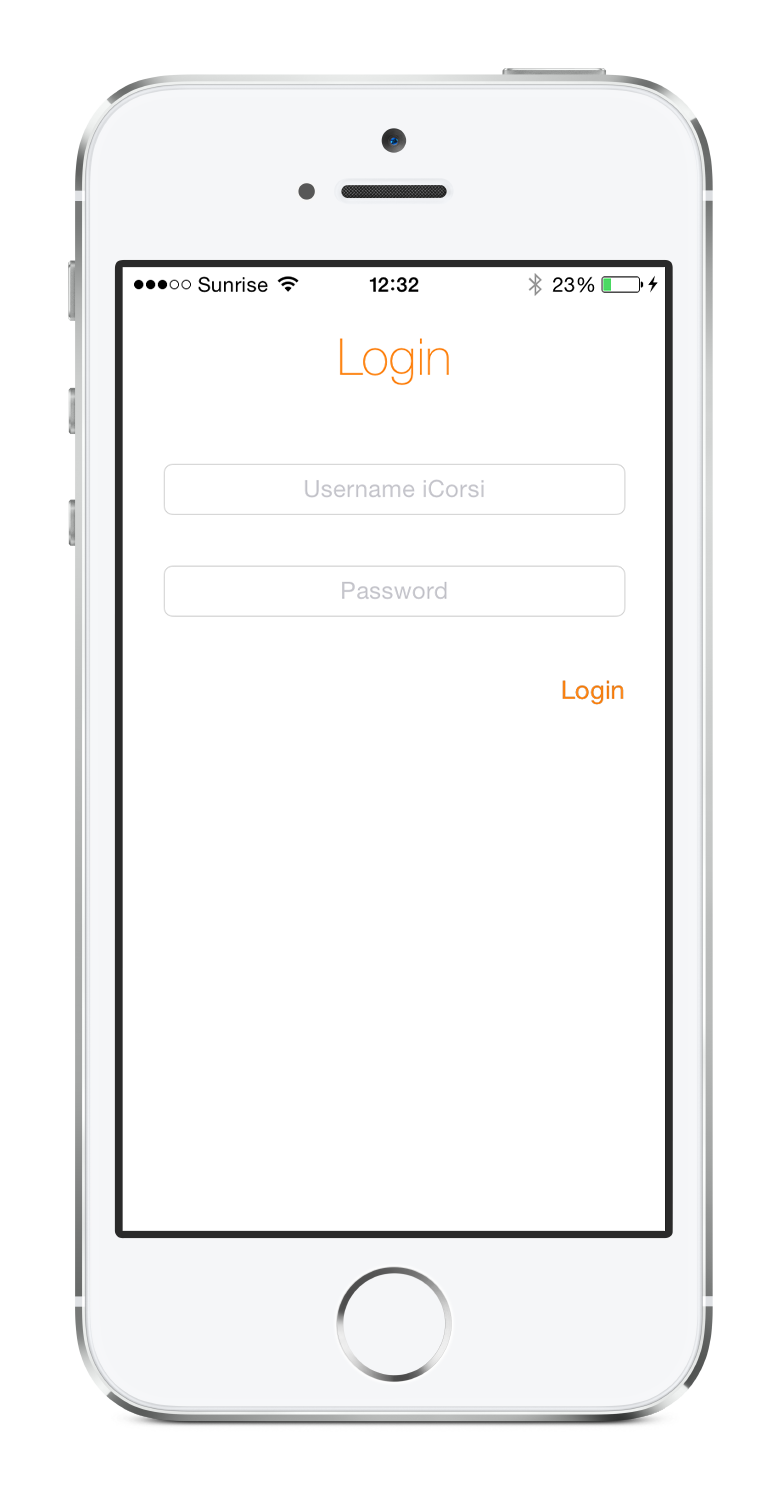
\includegraphics[scale=0.5]{img/iphone_login.png}
\caption{The login view of \UB\ }
\label{loginview}
\end{center}
\end{figure}

From then, the first technical step the user need to do is to \textbf{login} to the platform. We tried to keep the step as little as possible, saving the credential locally in the device once the login is successful.

\subsection{Outside behaviours}

The operations permitted to the user when he/she is outside the lecture room are the following:
\begin{itemize}
\item Login (stateless)
\item Search for the upcoming lectures
\item Choose the lectures he/she is going to attend
\item Start the position tracking
\item Chose a different upcoming lecture
\end{itemize}

\begin{figure}[htbp]
\begin{center}
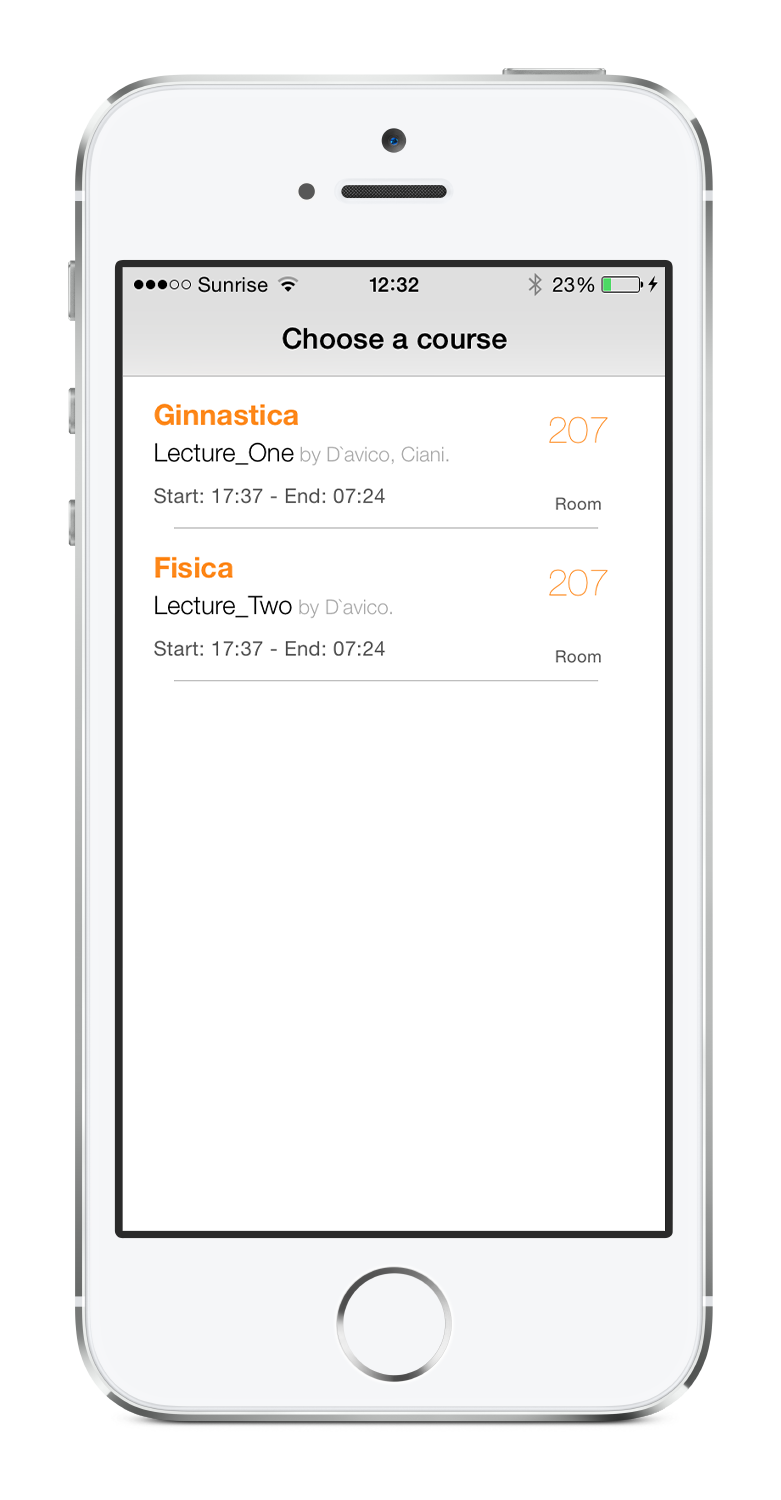
\includegraphics[scale=0.5]{img/iphone_courses.png}
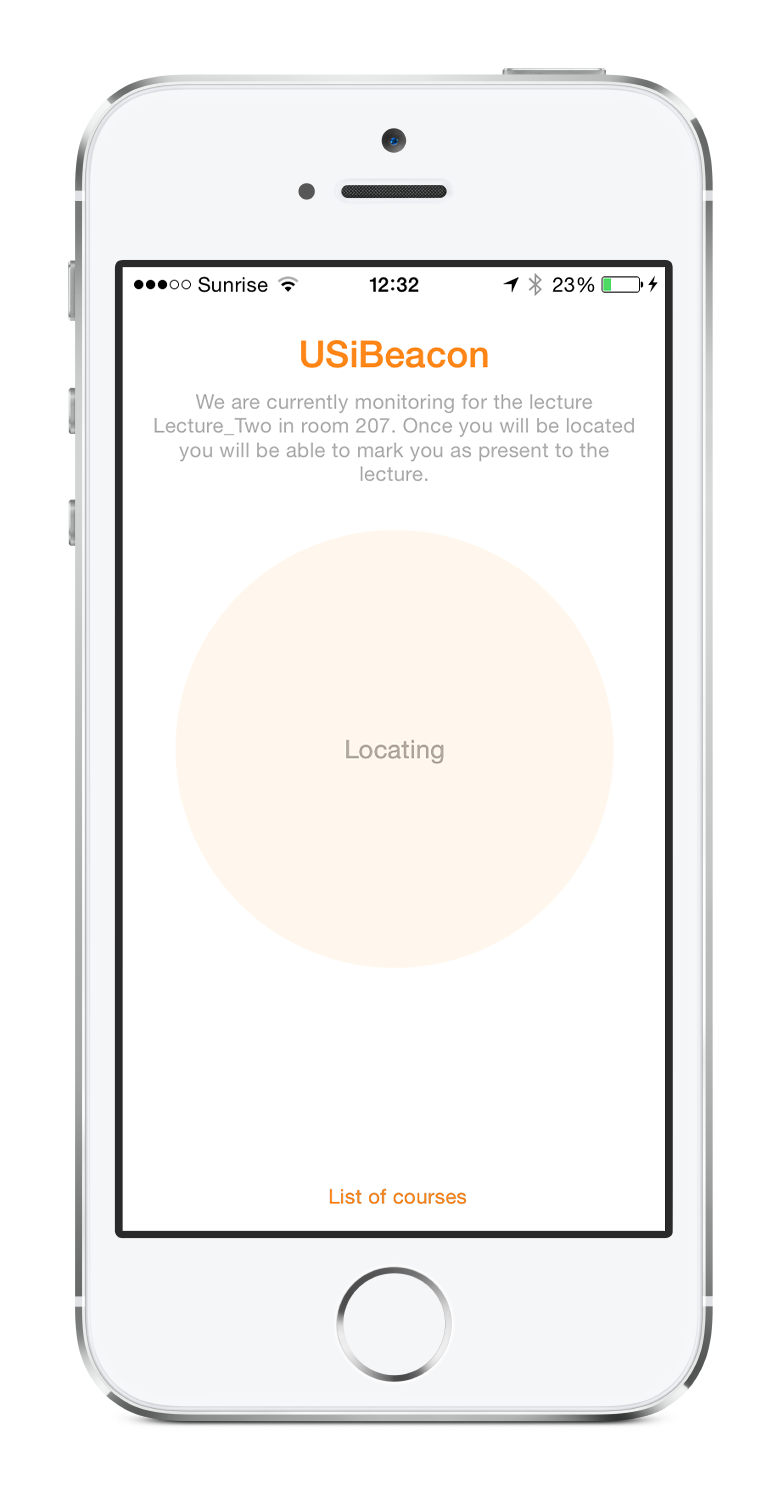
\includegraphics[scale=0.5]{img/iphone_locating.png}
\caption{The course selection (left) and the searching view (right)}
\label{courseselection}
\end{center}
\end{figure}

We chose to implement all these operation in a way that was as fast as possible: when the users open the application (and the are logged in) it automatically retrieves the list of the upcoming lectures that user should attend \textbf{within a time window of 15 minutes}.
If there is only one result the application will automatically go in ``tracking mode", starting to search for the room associated to that lecture, if instead the user has some overlaps (so there are multiple upcoming lectures) the application shows the course selection view (image \ref{courseselection} on the left) that permits the user to choose for which lecture start the tracking.\\

The last point (chose a different lecture) is achieved by a little button on the button of the searching view (image \ref{courseselection} on the right). This button permits to open again the course selection and choose a new lecture to track.

\subsection{Inside operation}
When the user move inside the room the application changes the behaviours permitting the user to \textbf{check in} to the lecture.\\

The application modifies the tracking view showing the checkin button as shown in figure \ref{checkinview}:

\begin{figure}[htbp]
\begin{center}
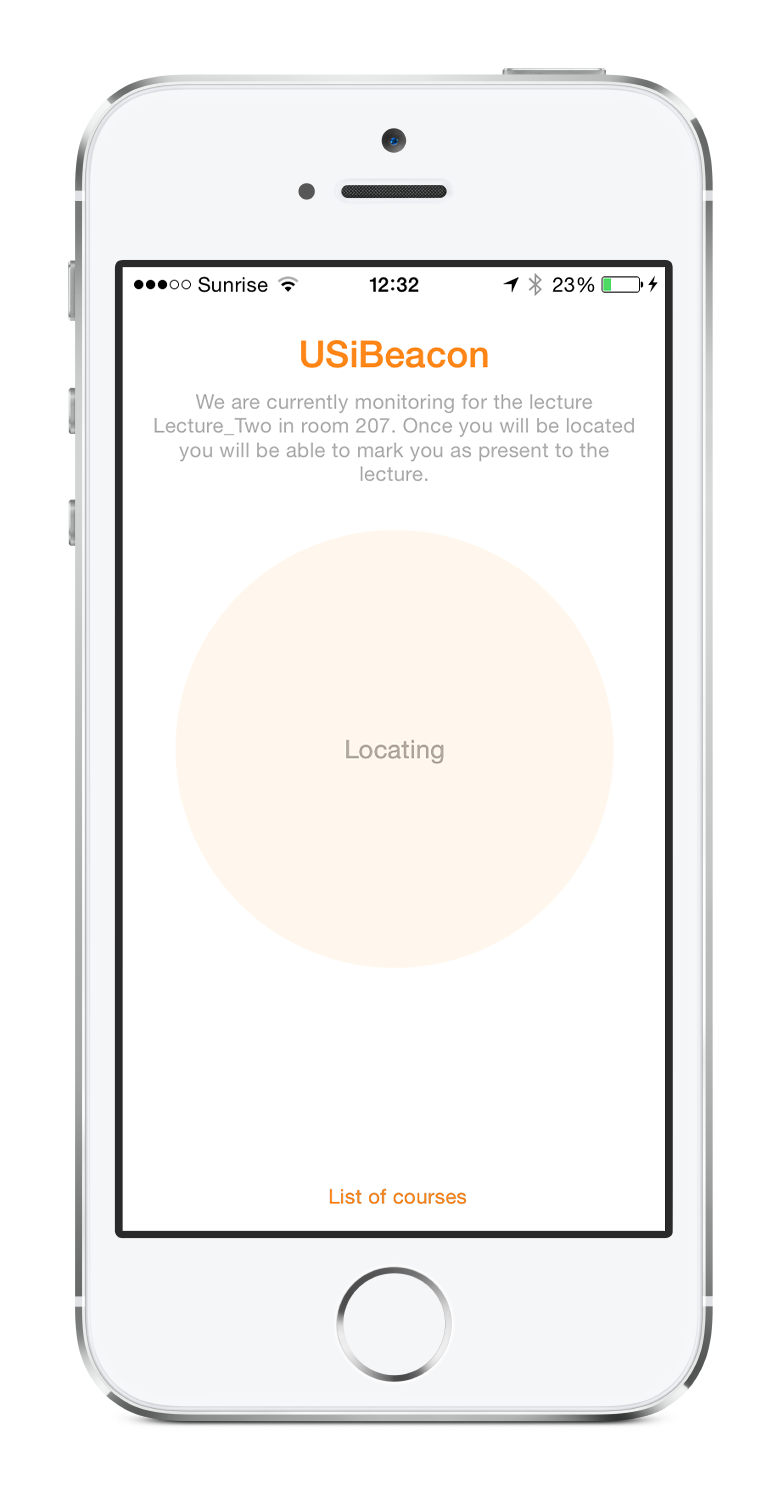
\includegraphics[scale=0.5]{img/iphone_locating.png}
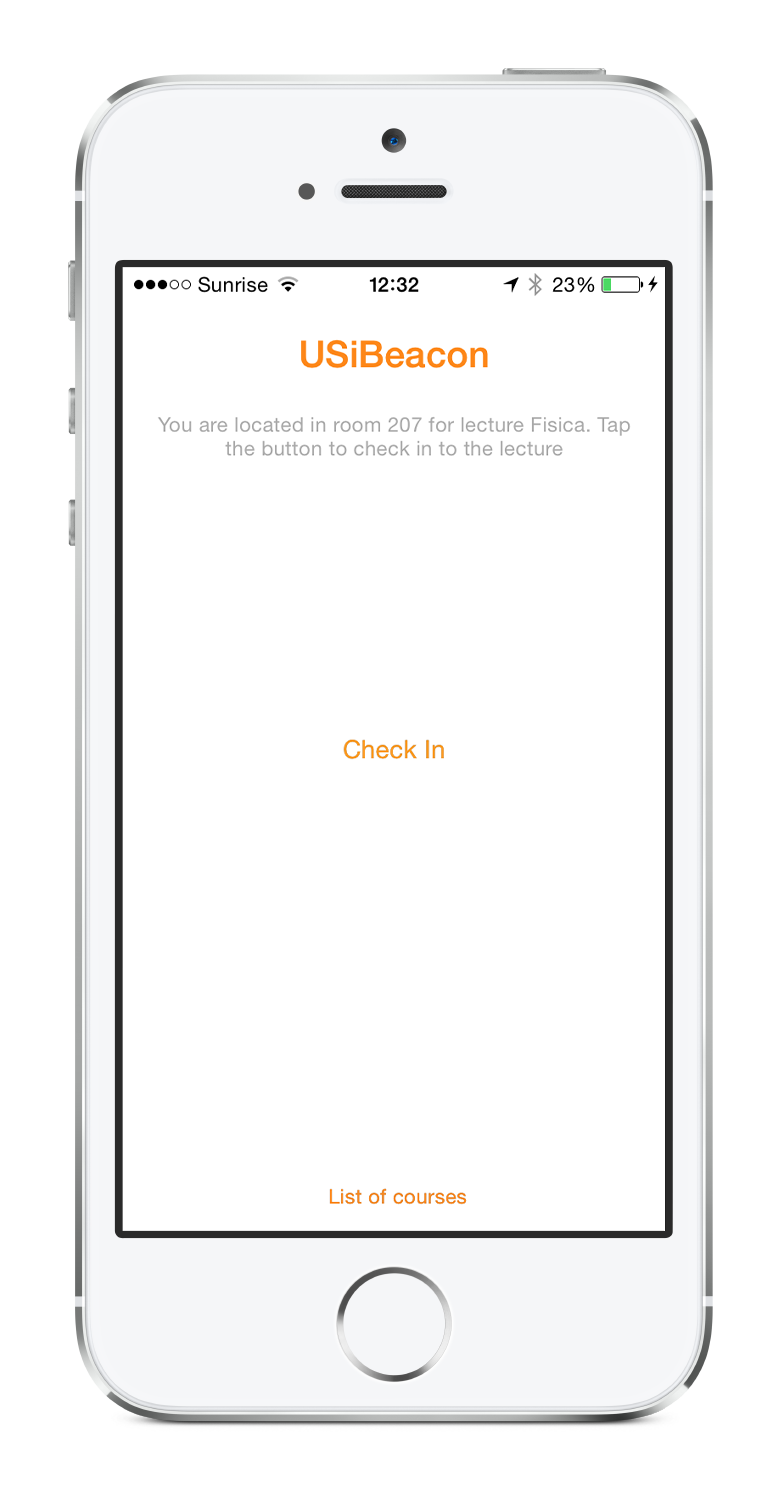
\includegraphics[scale=0.5]{img/iphone_founded.png}
\caption{The tracking view outside the room (left) and inside the tracked room (right)}
\label{checkinview}
\end{center}
\end{figure}

Once the user tap on the \emph{check in} button the application replies with the result of the checkin process that could be one of the following:
\begin{itemize}
\item \textbf{Successful:} The checkin process is concluded and the user is correctly signed to the lecture.
\item \textbf{Already Signed:} If the user tries to sign again to the same lecture a warning is visualised.
\item \textbf{Credential Error:} If the user is trying to checkin but his/her token is expired or the iCorsi password is changed an error is visualised and the user is \emph{not} signed to the lecture. In this case the login view (image \ref{loginview}) is visualised again to refresh the status.
\end{itemize}


\pagebreak

\section{The Dashboard}
\pagebreak

\section{The Dashboard}
\pagebreak



% 5. Reflections/ Discussion


\end{document}  